\documentclass[11pt, a4paper]{article}

\usepackage{amsmath, amssymb, titling}
\usepackage[margin=2.5cm]{geometry}
\usepackage[colorlinks=true, linkcolor=black, urlcolor=black, citecolor=black]{hyperref}
\usepackage{graphicx}
\usepackage{caption}
\usepackage{subcaption}
\usepackage{float}
\usepackage{cancel}
\usepackage{fancyhdr, lastpage}
\usepackage{fourier-orns}
\usepackage{xcolor}
\usepackage{nomencl}
\usepackage{etoolbox}
\makenomenclature

\setlength{\headheight}{18.2pt}
\setlength{\nomlabelwidth}{1.5cm}

\renewcommand\maketitlehooka{\null\mbox{}\vfill}
\renewcommand\maketitlehookd{\vfill\null}
\renewcommand{\headrule}{\vspace{-5pt}\hrulefill\raisebox{-2.1pt}{\quad\leafleft\decoone\leafright\quad}\hrulefill}
\newcommand{\parder}[2]{\frac{\partial {#1}}{\partial {#2}}}
\renewcommand\nomgroup[1]{%
  \item[\bfseries
  \ifstrequal{#1}{F}{Far--Away Properties}
]}

\title{Computational Fluid Dynamics \\ HW2}
\author{Almog Dobrescu\\\\ID 214254252}

\pagestyle{fancy}
\cfoot{Page \thepage\ of \pageref{LastPage}}

\begin{document}

\maketitle
\thispagestyle{empty}
\newpage

\thispagestyle{empty}
\tableofcontents
\vfil
\listoffigures
\newpage

\thispagestyle{empty}
\printnomenclature
\newpage

\setcounter{page}{1}
\section{Problem Definition}
\subsection{Governing Equations}
Consider the one-dimensional Navier-Stokes Equations:
\begin{equation}
    \frac{\partial Q}{\partial t}+\frac{\partial E}{\partial x}=\frac{\partial E_\nu}{\partial x}
\end{equation}
\nomenclature{$Q$}{conservation state space}
\nomenclature{$t$}{time}
\nomenclature{$E$}{inviscid convective vector}
\nomenclature{$E_\nu$}{viscous convective vector}
\nomenclature{$x$}{spatial coordinate}
Where:
\begin{equation}
    \begin{array}{c}
        \begin{matrix}
            Q=\begin{pmatrix}
                \rho \\\\
                \rho u \\\\
                e
            \end{pmatrix}, & E=\begin{pmatrix}
                \rho u \\\\
                p+\rho u^2 \\\\
                \left(e+p\right)u
            \end{pmatrix}, & E_\nu=\begin{pmatrix}
                0 \\\\
                \displaystyle\frac{4}{3}\mu\frac{\partial u}{\partial x} \\\\
                \displaystyle\frac{4}{3}\mu u\frac{\partial u}{\partial x}-\kappa\frac{\partial T}{\partial x}
            \end{pmatrix}
        \end{matrix} \\\\
        \begin{matrix}
            \displaystyle p=\left(\gamma-1\right)\left(e-\frac{1}{2}\rho u^2\right), & \displaystyle T=\frac{p}{\rho R}, \\\\
            \displaystyle\mu=1.458\cdot10^{-6}\frac{T^{\frac{3}{2}}}{T+110.4}, & \displaystyle\mu=2.495\cdot10^{-3}\frac{T^{\frac{3}{2}}}{T+194}
        \end{matrix} \\\\
        \begin{matrix}
            R=c_p-c_v, & \displaystyle\gamma=\frac{c_p}{c_v}
        \end{matrix}
    \end{array}
    \label{eq: definitions}
\end{equation}
\nomenclature{$\rho$}{fluid density}
\nomenclature{$u$}{fluid velocity}
\nomenclature{$e$}{total energy}
\nomenclature{$p$}{pressure}
\nomenclature{$\gamma$}{ratio of specific heats}
\nomenclature{$T$}{temperature}
\nomenclature{$R$}{gas constant}
\nomenclature{$\mu$}{coefficient of viscosity}
\nomenclature{$\kappa$}{coefficient of thermal conductivity}
\nomenclature{$c_p$}{constant specific heat capacity for a constant pressure}
\nomenclature{$c_v$}{constant specific heat capacity for a constant volume}
The constants are:
\begin{itemize}
    \item $\gamma=1.4$ for air under standard atmospheric conditions
    \item $R=287.0$ for air
\end{itemize}

\subsection{Physical Domain}
The physical domain is a tube extended between $x=0.2$ and $x=1.0$. At both ends there are impermeable walls.

\subsection{Initial Conditions}
The initial conditions are showen in Fig.\ref{fig: initial conditions}:
\begin{figure}[H]
    \centering
    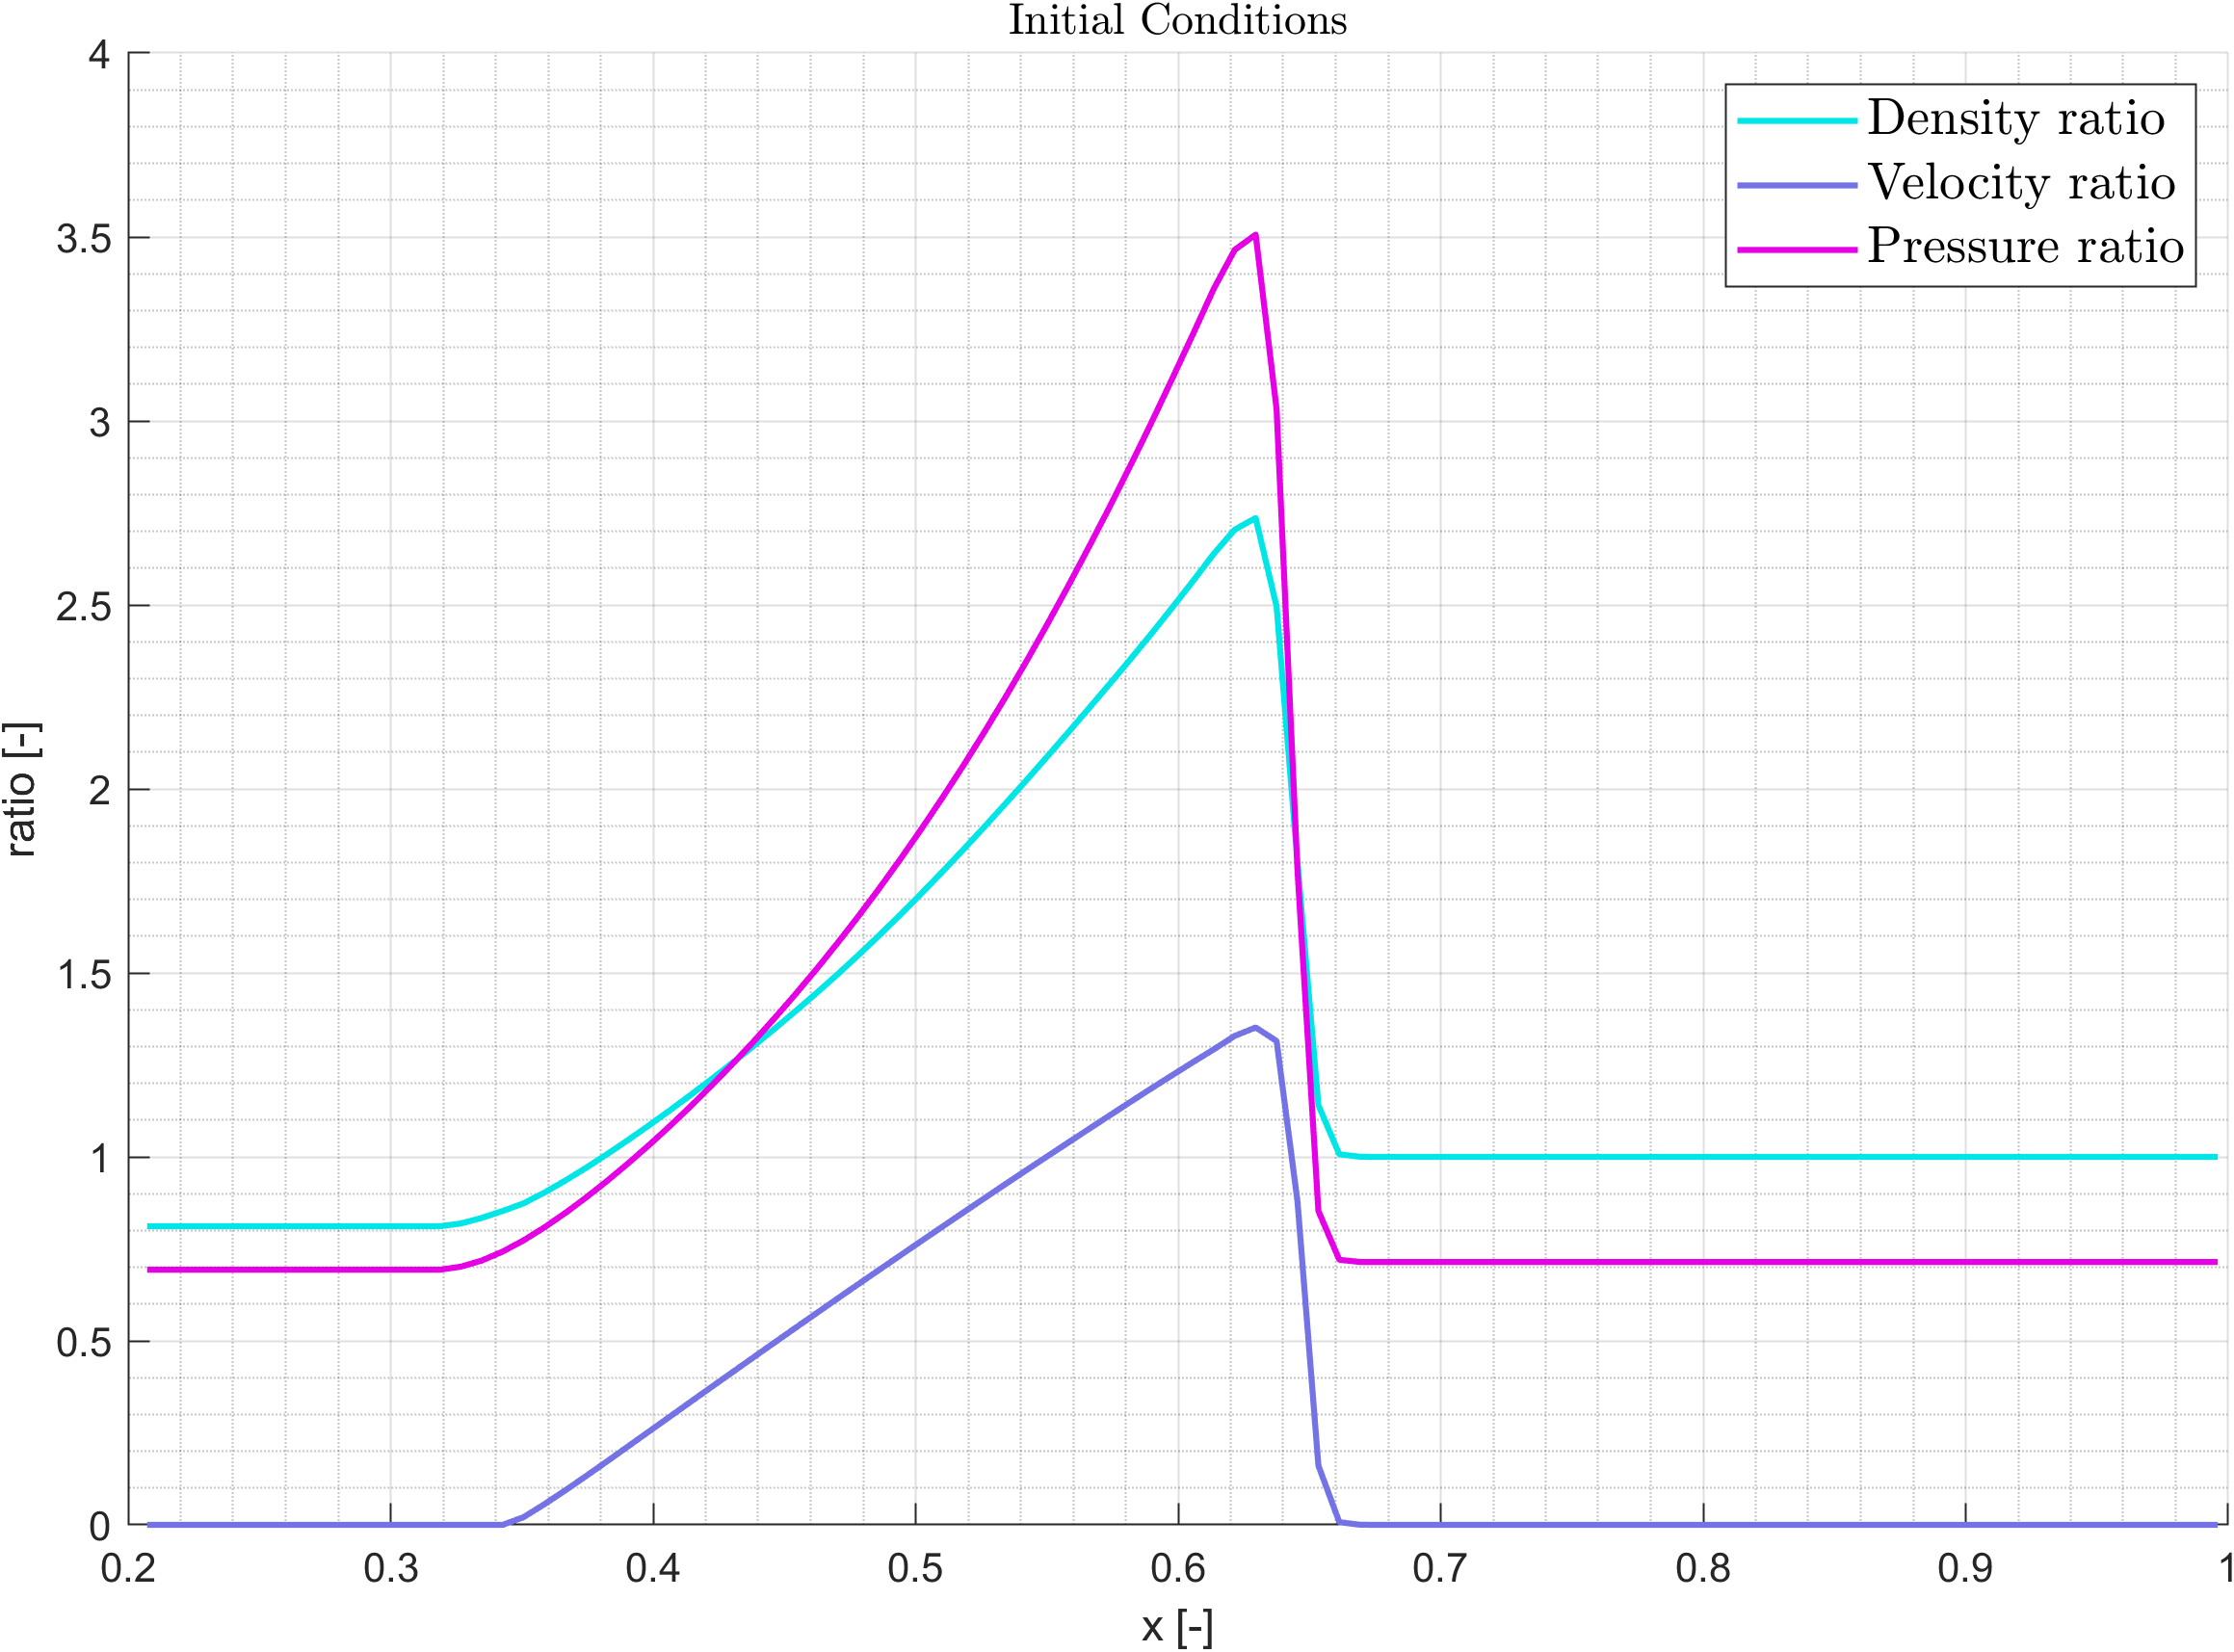
\includegraphics[width=0.4\textwidth]{images/Initial Conditions.png}
    \caption{Initial conditions}
    \label{fig: initial conditions}
\end{figure}

\subsection{Boundary Conditions}
On each side of the tube there is an adiabatic, soild wall boundary conditions. 
\begin{table}[H]
    \centering
    \begin{tabular}{cc||ccc||cc}
        $u_{\left(x=0.2\right)}=u_{\left(x=1.0\right)}=0$ &&& $\displaystyle\left.\frac{\partial p}{\partial x}\right|_{x=0.2}=\left.\frac{\partial p}{\partial x}\right|_{x=1.0}=0$ &&& $\displaystyle\left.\frac{\partial T}{\partial x}\right|_{x=0.2}=\left.\frac{\partial T}{\partial x}\right|_{x=1.0}=0$
    \end{tabular}
\end{table}

\section{Normalizing The Navier-Stokes Equations}
Since the initial conditions are normalized, there is a need to normaliz the N-S equations. We will use the following normalizations:
\begin{equation}
    \begin{matrix}
        \rho=\rho_\infty\tilde{\rho}, & u=a_\infty\tilde{u}, & p=\gamma p_\infty\tilde{p}, & T=\gamma T_\infty\tilde{T}, & x=L\tilde{x}, & \displaystyle t=\frac{L}{a_\infty}\tilde{t}, & \mu=\mu_\infty\tilde{\mu}, & \kappa=\kappa_\infty\tilde{\kappa}
    \end{matrix}
\end{equation}
\nomenclature[F]{$\rho_\infty$}{density far away}
\nomenclature[F]{$a_\infty$}{speed of sound far away}
\nomenclature[F]{$p_\infty$}{pressure far away}
\nomenclature[F]{$T_\infty$}{temperature far away}
\nomenclature[F]{$\mu_\infty$}{coefficient of viscosity far away}
\nomenclature[F]{$\kappa_\infty$}{coefficient of thermal conductivity far away}

\noindent The normalization of the temperature was choosen to cancel out the $\gamma$ in the normalization of the pressure:
\begin{equation}
    \begin{array}{lcl}
        p & = & \rho RT \\
        \gamma p_\infty\tilde{p} & = & \rho_\infty\tilde{\rho}R\gamma T_\infty\tilde{T} \\
        \tilde{p} & = & \tilde{\rho}\tilde{T}
    \end{array}
\end{equation}
The pressure normalization can be written also as:
\begin{equation}
    p=\gamma p_\infty\tilde{p}=\gamma\rho_\infty RT_\infty\tilde{p}=\rho_\infty a_\infty^2\tilde{p}
    \label{eq: normalization for pressure}
\end{equation}
From equations \ref{eq: definitions} and \ref{eq: normalization for pressure} we can derive the normalization for the energy:
\begin{equation}
    \begin{array}{lcl}
        e & = & \displaystyle\frac{p}{\gamma-1}+\frac{1}{2}\rho u^2 \\\\
        e & = & \displaystyle\frac{\rho_\infty a_\infty^2\tilde{p}}{\gamma-1}+\frac{1}{2}\rho_\infty\tilde{\rho}a_\infty^2\tilde{a}^2 \\\\
        e & = & \displaystyle \rho_\infty a_\infty^2\left(\frac{\tilde{p}}{\gamma-1}+\frac{1}{2}\tilde{\rho}\tilde{a}^2\right) \\\\
        e & = & \rho_\infty a_\infty^2\tilde{e}
    \end{array}
\end{equation}
% The normalizations for $\mu$ and $\kappa$ are there for:
% \begin{equation}
%     \begin{matrix}
%         \begin{array}{lcl}
%             \tilde{\mu} & = & \displaystyle\frac{\mu}{\mu_\infty}
%         \end{array} & \begin{array}{lcl}
%             \tilde{\kappa} & = & \displaystyle\frac{\kappa}{\kappa_\infty}
%         \end{array}
%     \end{matrix}
% \end{equation}
After substituting the normalizations in the N-S equations we get:
\begin{equation}
    \parder{}{\displaystyle\frac{L}{a_\infty}\tilde{t}}\begin{pmatrix}
        \rho_\infty\tilde{\rho} \\\\
        \rho_\infty a_\infty\tilde{\rho}\tilde{u} \\\\
        \rho_\infty a_\infty^2\tilde{e}
    \end{pmatrix}+\parder{}{L\tilde{x}}\begin{pmatrix}
        \rho_\infty a_\infty\tilde{\rho}\tilde{u} \\\\
        \rho_\infty a_\infty^2\tilde{p}+\rho_\infty a_\infty^2\tilde{\rho}\tilde{u}^2 \\\\
        \rho_\infty a_\infty^3\left(\tilde{e}+\tilde{p}\right)\tilde{u}
    \end{pmatrix}=\parder{}{L\tilde{x}}\begin{pmatrix}
        0 \\\\
        \displaystyle\frac{4}{3}\mu_\infty a_\infty\tilde{\mu} \parder{\tilde{u}}{L\tilde{x}} \\\\
        \displaystyle\frac{4}{3}\mu_\infty a_\infty^2\tilde{\mu}\tilde{u}\parder{\tilde{u}}{L\tilde{x}}-\frac{\kappa_\infty a_\infty^2}{R}\tilde{\kappa}\parder{\tilde{T}}{L\tilde{x}}
    \end{pmatrix}
\end{equation}
Rearranging:
\begin{equation}
    \frac{\rho_\infty a_\infty}{L}\parder{}{\tilde{t}}\begin{pmatrix}
        \tilde{\rho} \\\\
        a_\infty\tilde{\rho}\tilde{u} \\\\
        a_\infty^2\tilde{e}
    \end{pmatrix}+\frac{\rho_\infty a_\infty}{L}\parder{}{\tilde{x}}\begin{pmatrix}
        \tilde{\rho}\tilde{u} \\\\
        a_\infty\tilde{p}+a_\infty\tilde{\rho}\tilde{u}^2 \\\\
        a_\infty^2\left(\tilde{e}+\tilde{p}\right)\tilde{u}
    \end{pmatrix}=\frac{\mu_\infty}{L^2}\parder{}{\tilde{x}}\begin{pmatrix}
        0 \\\\
        \displaystyle\frac{4}{3}a_\infty\tilde{\mu} \parder{\tilde{u}}{\tilde{x}} \\\\
        \displaystyle\frac{4}{3}a_\infty^2\tilde{\mu}\tilde{u}\parder{\tilde{u}}{\tilde{x}}-\frac{\kappa_\infty a_\infty^2}{\mu_\infty R}\tilde{\kappa}\parder{\tilde{T}}{\tilde{x}}
    \end{pmatrix}
\end{equation}
Deviding the second equation by $a_\infty$, the third equation by $a_\infty^2$, and the whole set of equations by $\displaystyle\frac{\rho_\infty a_\infty}{L}$ we get:
\begin{equation}
    \parder{}{\tilde{t}}\begin{pmatrix}
        \tilde{\rho} \\\\
        \tilde{\rho}\tilde{u} \\\\
        \tilde{e}
    \end{pmatrix}+\parder{}{\tilde{x}}\begin{pmatrix}
        \tilde{\rho}\tilde{u} \\\\
        \tilde{p}+a_\infty\tilde{\rho}\tilde{u}^2 \\\\
        \left(\tilde{e}+\tilde{p}\right)\tilde{u}
    \end{pmatrix}=\frac{\mu_\infty}{L\rho_\infty a_\infty}\parder{}{\tilde{x}}\begin{pmatrix}
        0 \\\\
        \displaystyle\frac{4}{3}\tilde{\mu} \parder{\tilde{u}}{\tilde{x}} \\\\
        \displaystyle\frac{4}{3}\tilde{\mu}\tilde{u}\parder{\tilde{u}}{\tilde{x}}-\frac{\kappa_\infty}{\mu_\infty R}\tilde{\kappa}\parder{\tilde{T}}{\tilde{x}}
    \end{pmatrix}
\end{equation}
The Reynolds number and the mach number far away are defined as:
\begin{equation}
    \begin{array}{c}
        \begin{matrix}
            \displaystyle M_\infty=\frac{u_\infty}{a_\infty} & \displaystyle Re_{L\infty}=\frac{\rho_\infty u_\infty L}{\mu_\infty}
        \end{matrix} \\
        \Downarrow \\
        \displaystyle \frac{\mu_\infty}{L\rho_\infty a_\infty}=\frac{M_\infty}{Re_{L\infty}}
    \end{array}
\end{equation}
\nomenclature[F]{$M_\infty$}{mach number far away}
\nomenclature[F]{$Re_{L\infty}$}{Reynolds number with respect to L far away}
The Prandtl number far away is defined as:
\begin{equation}
    \begin{array}{c}
        \displaystyle Pr_\infty=\frac{c_p\mu_\infty}{\kappa_\infty} \\
        \Downarrow \\
        \displaystyle\frac{\kappa_\infty}{\mu_\infty R}=\frac{c_p}{Pr_\infty \left(c_p-c_v\right)}=\frac{\gamma}{Pr_\infty\left(\gamma-1\right)}
    \end{array}
\end{equation}
\nomenclature[F]{$Pr_\infty$}{Prandtl number far away}
Substituting into the normalized N-S equations:
\begin{equation}
    \parder{\tilde{Q}}{\tilde{t}}+\parder{\tilde{E}}{\tilde{x}}=\frac{M_\infty}{Re_{L\infty}}\parder{\tilde{E}_\nu}{\tilde{x}}
\end{equation}
Where:
\begin{equation}
    \begin{matrix}
        \tilde{Q}=\begin{pmatrix}
        \tilde{\rho} \\\\
        \tilde{\rho}\tilde{u} \\\\
        \tilde{e}
        \end{pmatrix}, & \tilde{E}=\begin{pmatrix}
        \tilde{\rho}\tilde{u} \\\\
        \tilde{p}+a_\infty\tilde{\rho}\tilde{u}^2 \\\\
        \left(\tilde{e}+\tilde{p}\right)\tilde{u}
        \end{pmatrix}, & \tilde{E_\nu}=\begin{pmatrix}
        0 \\\\
        \displaystyle\frac{4}{3}\tilde{\mu} \parder{\tilde{u}}{\tilde{x}} \\\\
        \displaystyle\frac{4}{3}\tilde{\mu}\tilde{u}\parder{\tilde{u}}{\tilde{x}}-\frac{\gamma}{Pr_\infty\left(\gamma-1\right)}\tilde{\kappa}\parder{\tilde{T}}{\tilde{x}}
        \end{pmatrix}
    \end{matrix}
\end{equation}

\section{The Computational Domain}
\subsection{Discretization}
The physical domain $\left[x_I,x_F\right]$ is discretizes into N equispaced cells. The size of each cell is there for:
\begin{equation}
    \Delta x=\frac{x_F-x_I}{N}=\frac{L}{N}
\end{equation}
\nomenclature{$x_F$}{x coordinate of the end of the domain}
\nomenclature{$\Delta x$}{size of each cell in the domain}
\nomenclature{$L$}{characteristic length}
so the x coordinate of the i-th cell $x_i$ is:
\begin{equation}
    \begin{matrix}
        \displaystyle x_i=x_I+\frac{1}{2}\Delta x+\Delta x\cdot\left(i-1\right) && \text{when starting from $i=1$}
    \end{matrix}
\end{equation}
\nomenclature{$x_i$}{x coordinate of the i-th cell}

\subsection{Boundary Conditions}
In order to set the boundary conditions on the edge faces we will define ghost cells that will be calculated like so:
\begin{equation}
    \begin{array}{lcl}
        u_{\left(i=0\right)} &=& -u_{\left(i=1\right)} \\
        u_{\left(i=N+1\right)} &=& -u_{\left(i=N\right)}
    \end{array}
    \label{eq: velocity boundary}
\end{equation}
in order to mentain velocity zero on the boundary and like so:
\begin{equation}
    \begin{array}{lcl}
        T_{\left(i=0\right)} &=& T_{\left(i=1\right)} \\
        T_{\left(i=N+1\right)} &=& T_{\left(i=N\right)}
    \end{array}
    \label{eq: temp boundary}
\end{equation}
in order to mentain adiabatic boundary conditions.
Since the gradient of the pressure on the wall is zero, we get:
\begin{equation}
    \begin{array}{lcl}
        p_{\left(i=0\right)} &=& p_{\left(i=1\right)} \\
        p_{\left(i=N+1\right)} &=& p_{\left(i=N\right)}
    \end{array}
    \label{eq: pressure boundary}
\end{equation}
From equations \ref{eq: definitions}, \ref{eq: temp boundary}, and \ref{eq: pressure boundary} we can conclude:
\begin{equation}
    \begin{array}{lcl}
        \rho_{\left(i=0\right)} &=& \rho_{\left(i=1\right)} \\
        \rho_{\left(i=N+1\right)} &=& \rho_{\left(i=N\right)}
    \end{array}
    \label{eq: density boundary}
\end{equation}
and from equations \ref{eq: definitions}, \ref{eq: velocity boundary}, \ref{eq: pressure boundary}, and \ref{eq: density boundary} we can conclude:
\begin{equation}
    \begin{array}{lcl}
        e_{\left(i=0\right)} &=& e_{\left(i=1\right)} \\
        e_{\left(i=N+1\right)} &=& e_{\left(i=N\right)}
    \end{array}
    \label{eq: energy boundary}
\end{equation}
\newpage

\section{The Numerical Schemes}

\subsection{First Order Approximate Riemann Roe Method}

\subsection{First Order Steger-Warming -- Explicit}

\subsection{First Order Steger-Warming -- Implicit}

\end{document}